%\documentclass{article}
%\usepackage{amsmath, amsthm, amssymb}
%\usepackage{graphicx}
%\usepackage{algorithm}

\RequirePackage{etoolbox}
\csdef{input@path}{%
 {sty/}% cls, sty files
 {img/}% eps files
}%
\csgdef{bibdir}{bib/}% bst, bib files

\documentclass[ba]{imsart}
%
\pubyear{0000}
\volume{00}
\issue{0}
\doi{0000}
\firstpage{1}
\lastpage{1}


%
\usepackage{amsthm}
\usepackage{amsmath}
\usepackage{natbib}
\usepackage[colorlinks,citecolor=blue,urlcolor=blue,filecolor=blue,backref=page]{hyperref}
\usepackage{graphicx}
\usepackage[utf8]{inputenc}
\usepackage{amssymb}
\usepackage{enumerate}
\usepackage{verbatim}
\usepackage{booktabs}
\usepackage[ruled,vlined]{algorithm2e}
\usepackage{algpseudocode}
\usepackage{color}
\usepackage{dsfont}
\usepackage{float}

\startlocaldefs
% ** Local definitions **
\endlocaldefs

\setlength\parindent{0pt}
\newcommand{\iidsim}{\stackrel{iid}{\sim}}

\begin{document}

%\maketitle
%\title{}
\date{April 2020}

\begin{frontmatter}
\title{Discussion of ``Unified Framework for De-Duplication and Population Size Estimation'' by Tancredi et al.}
\subtitle{\large (report on code and experiments)}
%\title{\thanksref{T1}}
%\thankstext{T1}{<thanks text>}
\runtitle{}

\begin{aug}
\author{\fnms{Nianqiao}~\snm{Ju}\thanksref{addr1,t1} \ead[label=e1]{nju@g.harvard.edu}},
\author{\fnms{Niloy}~\snm{Biswas}\thanksref{addr1}},
\author{\fnms{Pierre E.}~\snm{Jacob} \thanksref{addr1}},
\author{\fnms{Gonzalo}~\snm{Mena} \thanksref{addr1,addr2}},
\author{\fnms{John}~\snm{O'Leary}\thanksref{addr1}}
\and
\author{\fnms{Emilia}~\snm{Pompe}\thanksref{addr3}}
%\author{\fnms{<firstname>} \snm{<surname>}\thanksref{}\ead[label=e1]{}}
%\and
%\author{\fnms{} \snm{}}
\runauthor{Ju et al.}

\address[addr1]{Department of Statistics, Harvard University 
}

\address[addr2]{Harvard Data Science Initiative}

\address[addr3]{Department of Statistics, University of Oxford}
\thankstext{t1}{\printead{e1}}
%\thankstext{<id>}{<text>}
\end{aug}


\begin{abstract}
This document is a draft of the documentation
for the code available at
\url{https://github.com/EmiliaPompe/discussion_unified_framework}.
We describe the model of Tancredi, Steorts and Liseo,
briefly and then proceed to describing
implementation choices, and some numerical results.
\end{abstract}
\end{frontmatter}

\section{Context, model and target distribution}

We consider a de-duplication task on a dataset $v$, as in Tancredi et al. While $v$ could potentially contain several distinct files, for simplicity we assume that we have exactly one file with records $j \in \{1,\dots,n\}$ and fields $\ell \in \{1, \dots, p \}$, taking values ${v_{j,\ell} \in \{1, \dots, M_\ell\}}$.
We think of $v$ as a corrupted version of an unobserved dataset with $N$ distinct records, where $N$ is unknown.
The model relating $v$ to this unobserved dataset involves a few components:
\begin{itemize}
    \item A mechanism to link the $n$ observed records to the $N$ unobserved records, whereby more than one observed record might relate to the same unobserved record. Thus we are talking about a model of partitions of $\{1,\ldots,n\}$.
    \item A mechanism for the corruption process linking the observed and underlying data.
    \item A model component related to $N$, the latent population size.
\end{itemize}

%The paper introduces a bunch of objects but then replaces some of them by others when it comes to the sampling algorithm. Here let's focus on what's useful for the sampling algorithm.

We write $p(\eta, N, \beta', \beta_0, \theta)$ for the target distribution, leaving its dependence on the observations $v$ implicit. Here $\eta$ describes the partition associating observed records with unique underlying entities; in particular, $\eta$ is a $n$-vector with $\eta_j \in \{1,\ldots,n\}$ for $j \in \{1,\dots,n\}$.
For the other variables $N \in \mathbb{N}$ denotes the true population size, $\beta',\beta_0$ are associated with the corruption mechanism, and $\theta$ describes the frequency of each field value among the unobserved records. Thus for each $\ell \in \{1,\dots,p\}$, $\theta_\ell$ is a vector of probabilities on the set $\{1,\dots,M_\ell\}$.

Although we can describe any partition of $\{1, \dots, n\}$ with an $\eta$ as described above, it will be convenient to have an alternative description of the partition for the computations below. In particular, we note that there is a bijection relating each possible $\eta$ with a pair $(Z,U')$, where $Z$ contains $k(Z)$ blocks of indices and $U'$ is a list of $k(Z)$ labels.
Observations $i$ and $j$ belong to the same block in $Z$ exactly when $\eta_i = \eta_j$, and this common $\eta$ value corresponds to the label of this block in $U'$.
For example, if $\eta = (3,1,2,5,3)$ then $Z = (15|2|3|4)$, $U'=(3,1,2,5)$, and $k(Z) = 4$. We write $U = (u_z^\prime)$, so that block $z \in Z$ has label $u_z^\prime$.
%Note that the labels in $U'$ take values in $\{1,\ldots,n\}$ but there are only $N$ unique values at most, because $Z$ has at most $N$ blocks (according to the prior specification recalled below).

We take the target distribution to be
\begin{align}
    & p(\eta, N, \beta', \beta_0, \theta)\nonumber \\
    & = \Big( \prod_{z\in Z} p(v_z|Z,U',N,\beta',\theta) \Big) p(U'|Z,N)p(Z|N)p(N)p(\beta'|\beta_0) p(\beta_0) p(\theta). \label{eq:posteriorfactorization}
\end{align}
We describe each part of this equation in turn, below.
Here the right hand side involves $(Z,U')$ instead of $\eta$, but this is unproblematic due to the bijection described above. 
The term $v_z$ refers to the set of observations $(v_i)$ for $i\in z$. 

First, the prior $p(\theta)$ follows the Dirichlet distribution.
The prior $p(\beta_0)$ specifies that the components $\beta_{0,\ell} \iidsim \mathcal{N}(m_0, s_0^2)$, with $m_0=\text{logit}(0.01)$ and $s_0^2 = 0.1$. The conditional prior $p(\beta' | \beta_0)$ is that 
$\beta'_{j,\ell} \iidsim \mathcal{N}(\beta_{0,\ell},s^2)$
for $j\in\{1,\ldots,n\}$. We set $s^2 = 0.5$, as suggested by 
Tancredi et al.
The prior on population size is $p(N)\propto N^{-g}$ for some $g$, and again following the authors we set $g=1.02$.

Given $N$, we assume $(Z,U')$ has prior
\begin{equation}
\label{eq:priorZU}
    p(Z,U'|N) = p(U'|Z,N)\times p(Z|N) = \frac{1}{n_k} \frac{N_k}{N^n}.
\end{equation}
Here we write $a_b := a!/(a-b)!$ for any pair of integers $a\geq b$, and $k = k(Z)$, the number of blocks in $Z$. We note that the conditional distribution of $Z$ given $N$ is supported on partitions with at most $N$ blocks.

We now consider the term $p(v_z|Z,U',N,\beta',\theta)$, which can be interpreted as the likelihood associated with block $z$ of partition $Z$.  We first assume that this factorizes into a product of $p$ terms corresponding to each data field, so that
\begin{equation}
p(v_z|Z,U',N,\beta',\theta) = \prod_{\ell=1}^p p(v_{z,\ell}|Z,U',N,\beta',\theta).
\label{eq:productoverfields}
\end{equation}
In the following the label, we will identify the label $u'_z$ with one of the $N$ latent records in $\tilde{v}$, where each $\tilde{v}_{u'_z}$ is a $p$-dimensional vector of data items.
Note that this involves a minor abuse of notation, since $u'_z$ refers to one of the $N$ underlying records while the value of its label might not fall in $\{1,\ldots,N\}$ if $N < n$. Nevertheless we can 
treat $\tilde{v}_{u'_z}$ as the component of $\tilde{v}$ associated with block $z$, as long as there are fewer than $N$ 
unique values among $(\eta_j)_{j\in 1:n}$.

In the following we fix a particular $\ell$, noting that the same calcuations will hold for any $\ell \in \{1, \dots, p\}$. 
For any observation $j \in  \{1, \dots, n\}$ and data item $\ell \in \{1, \dots, p\}$, we also 
define ${\alpha'_{j,\ell} := \text{expit}(\beta'_{j,\ell}) = \exp(\beta'_{j,\ell})/(1+\exp(\beta'_{j,\ell}))}$, recalling that $\beta'$ is a vector parameterizing the data corruption mechanism.

By introducing $\tilde{v}_{u'_z,\ell}$ and simplifying the notation by removing unnecessary objects in the conditioning, we can write
\begin{equation}
p(v_{z,\ell}|Z,U',N,\beta',\theta) = \sum_{\tilde{v}_{u'_z,\ell}}     
p(v_{z,\ell}|\tilde{v}_{u'_z,\ell},\beta'_{u'_z,\ell},\theta) p(\tilde{v}_{u'_z,\ell}|\theta),
\end{equation}
the sum running over the $M_\ell$ possible values of $\tilde{v}_{u'_z,\ell}$.
We have $p(\tilde{v}_{u'_z,\ell}|\theta) = \theta_{\ell,\tilde{v}_{u'_z,\ell}}$ under the Categorical distribution.
The term $p(v_{z,\ell}|\tilde{v}_{u'_z,\ell},\beta'_{u'_z,\ell},\theta)$ describes the corruption mechanism associated with the underlying record labelled $u'_z$ and $\ell$-th entry.
If $z$ contains just one index, say $j\in\{1,\ldots,n\}$,
we have 
\[
p(v_{j,\ell}|\tilde{v}_{u'_z,\ell},\beta'_{u'_z,\ell},\theta) = (1-\alpha'_{u'_z,\ell})\mathds{1}(\tilde{v}_{u'_z,\ell} = v_{j,\ell})
+ \alpha'_{u'_z,\ell} \theta_{\ell v_{j,\ell}},
\]
thus multiplying by $\theta_{\ell,\tilde{v}_{u'_z,\ell}}$ and summing over $\tilde{v}_{u'_z,\ell}$ in $\{1,\ldots,M_\ell\}$, and recalling
that the sum of the entries of $\theta_\ell$ is one, we obtain 
\[(1-\alpha'_{u'_z,\ell}) \times \theta_{\ell,v_{j,\ell}}
+ \alpha'_{u'_z,\ell} \theta_{\ell,v_{j,\ell}} = \theta_{\ell,v_{j,\ell}}.\]
Thus if $z = \{j\}$ we have 
\begin{equation}
p(v_{z,\ell}|Z,U',N,\beta',\theta) = \theta_{\ell,v_{j,\ell}}.
\label{eq:case_singleton}
\end{equation}

Next, consider the case where block $z$ contains
two indices, $z = \{j_1,j_2\}$.
We can differentiate between two cases: $v_{j_1,\ell} = v_{j_2,\ell}$ and  
$v_{j_1,\ell} \neq v_{j_2,\ell}$, and introduce the latent variable $\tilde{v}_{u'_z,\ell}$ as previously. 
In the former case, for any $\tilde{v}_{u'_z,\ell}$ among $M_\ell$ possible values,
\begin{align*}
    &p(v_{z,\ell}|\tilde{v}_{u'_z,\ell},Z,U',N,\beta',\theta)\\
    &= p(v_{j_1,\ell}|\tilde{v}_{u'_z,\ell},\beta'_{u'_z,\ell},\theta)
    \times p(v_{j_2,\ell}|\tilde{v}_{u'_z,\ell},\beta'_{u'_z,\ell},\theta)\\
    &= (1-\alpha^{'2}_{u'_z,\ell}) \mathds{1}(\tilde{v}_{u'_z,\ell} = v_{j_1,\ell}) \\
    &+ 2 (1-\alpha'_{u'_z,\ell}) \alpha'_{u'_z,\ell} \theta_{\ell, v_{j_1,\ell}} \mathds{1}(\tilde{v}_{u'_z,\ell} = v_{j_1,\ell}) \\ 
    &+ \alpha^{'2}_{u'_z,\ell} \theta_{\ell, v_{j_1,\ell}}^2,
\end{align*}
thus multiplying by $\theta_{\ell,\tilde{v}_{u'_z,\ell}}$ and summing over $\tilde{v}_{u'_z,\ell}$ in $\{1,\ldots,M_\ell\}$, we obtain
\begin{align*}
p(v_{z,\ell}|Z,U',N,\beta',\theta) &= (1-\alpha'_{u'_z,\ell})^2 \theta_{\ell,v_{j_1,\ell}} \\ 
&+ (2\alpha'_{u'_z,\ell}-\alpha^{'2}_{u'_z,\ell}) \theta_{\ell, v_{j_1,\ell}}^2,
\end{align*}
while if $v_{j_1,\ell} \neq v_{j_2,\ell}$ we obtain 
\begin{align*}
p(v_{z,\ell}|Z,U',N,\beta',\theta) &=
(2\alpha'_{u'_z,\ell}-\alpha^{'2}_{u'_z,\ell}) \theta_{\ell, v_{j_1,\ell}}\theta_{\ell, v_{j_2,\ell}}.
\end{align*}
At the end of the day we obtain the same formula as in Section 4 of the article (bottom of page 11),
with $\beta,U$ replaced by $\beta',U'$. The recursion formula is as follows,
for a block $z$ that contains an index $j^\star$ and $s-1$ others denoted by $j_1,\ldots,j_{s-1}$,
\begin{equation}
    \label{eq:recursion}
    \begin{split}
        &p(v_{z,\ell}|Z,U',N,\beta',\theta) =
        \alpha'_{u'_z, \ell} \theta_{\ell, v_{j^\star,\ell}}
        p(v_{z\setminus\{j^\star\}, \ell}|Z,U',N,\beta', \theta) \\
        &+ (1-\alpha'_{u'_z, \ell}) \theta_{\ell,v_{j^\star,\ell}} 
        \prod_{h=1}^{s-1} \left[ (1-\alpha'_{u'_z, \ell})\mathds{1}(v_{j_h,\ell}=v_{j^\star,\ell}) + \alpha'_{u'_z, \ell} \theta_{\ell,v_{j_h,\ell}}\right].
    \end{split}
\end{equation}
This is a key formula for the implementation
of the Gibbs sampler.

Note that the derivatives of the likelihood 
$p(v_{z,\ell}|Z,U',N,\beta',\theta)$
could be also computed, for fixed $Z,U',N$, with respect to $\theta$
and with respect to $\beta'$, using similar recursions.
This could be used to perform gradient-based MCMC 
updates for these components.

\section{Conditional distributions and Gibbs sampling}

The algorithm operates on the variables
$(\eta, \beta', N, \beta_0, \theta)$. The target
distribution is provided in equation \eqref{eq:posteriorfactorization}. 
%[note: same as ]
%\begin{equation}
%    \label{eq:joint_posterior}
%    p(\eta, N, \beta',\beta_0,\theta) \propto \prod_{z \in Z}p(\nu_z \mid Z, U', %\beta'_{u'_z},\theta)\cdot p(U' \mid Z, N) \cdot p(Z\mid N) \cdot p(\beta' \mid %\beta_0) p(N) p(\beta_0) p(\theta).
%\end{equation}
We can draw samples from this distribution by updating the elements 
$\eta, \beta', \beta_0,N$ and $\theta$ with a Gibbs sampler, 
iteratively targeting the conditional distributions of each of these
variables given the others.


\subsection{Draw $\eta$ given the rest}

To begin, we describe the update of the labels $\eta = (Z, U')$ given the other variables. We do so by
updating each $\eta_j$ in turn, given the other labels $\eta_{-j}$ and the other state variables.
For each possible label value $q \in \{1,\ldots,n\}$
%in our implementation but with the additional note that
%there must be at most $N$ distinct labels,
we compute the probability of $\{\eta_j = q\}$
under the full conditional distribution as
\begin{equation}
    \label{eq:conditional_eta}
    \mathbb{P}\left(\eta_j = q \mid \eta_{-j}, N, \beta',\beta_0, \theta, v\right) \propto
    \frac{p(v_{z_q}\mid \eta, \beta'_q,\theta)}{p(v_{z_{q}\setminus\{j\}}\mid \eta, \beta'_q,\theta)}
    \mathbb{P}\left(\eta_j = q \mid \eta_{-j}\right).
\end{equation}

Here $z_q$ refers to the partition block with label
$q$, i.e. $u'_{z_q} = q$, so that the block $z_q$
contains all indices $j$ such that $\{\eta_j = q\}$.
The leading factor in~\eqref{eq:conditional_eta} can be interpreted as a
likelihood ratio, with the right-most term coming from the prior. This is equation (5.5) in the paper. The likelihood ratio can be computed using
\eqref{eq:productoverfields} and \eqref{eq:case_singleton}
%\begin{align}
%    \frac{p(\nu_{z_q}\mid \eta,
%\beta'_q,\theta)}{p(\nu_{z_{q}\setminus\{j\}}\mid \eta, \beta'_q,\theta)}
%    &= \prod_{\ell=1}^p \theta_{\ell,v_{j,\ell}}
%\end{align}
if $q$ identifies a new block and
otherwise following \eqref{eq:recursion} given $p(v_{z_q\setminus\{j\}}|\eta,\beta'_q,\theta)$.



\begin{comment}
{\color{red} Is the following correct?}
The prior leads to 
$\mathbb{P}\left(\eta_j = q \mid \eta_{-j}\right)=1/(n-k_{-j})$ if $q$ identifies an existing cluster and  
$\mathbb{P}\left(\eta_j = q \mid \eta_{-j}\right)=1/(n-k_{-j})$ in case of a new cluster, leading
to a probability of $(N-k_{-j})/(n-k_{-j})$ of a new cluster. Here $k_{-j}$ refers to the number
of clusters in the partition obtained from $\eta_{-j}$.
\end{comment}

To compute the $\mathbb{P}\left(\eta_j = q \mid \eta_{-j}\right)$ term in \eqref{eq:conditional_eta}, 
we can use \eqref{eq:priorZU}. Denote by $k^-$ the number of clusters in $\eta_{-j}$. Then,
\begin{flalign*}
\mathbb{P}\left(\eta_j = q \mid \eta_{-j}\right) & \propto \mathbb{P}\left(\eta_j = q, \eta_{-j}\right) \\
& = \left\{\begin{matrix}
\frac{1}{n_{k^-}} \frac{N_{k^-}}{N^n} & \text{if $q$ in an existing cluster}\\ 
\frac{1}{n_{k^-+1}} \frac{N_{k^-+1}}{N^n} & \text{if $q$ in a new cluster}
\end{matrix}\right. \\
&\propto \left\{\begin{matrix}
1 & \text{if $q$ in an existing cluster}\\ 
\frac{N-k^-}{n - k^-} & \text{if $q$ in a new cluster}
\end{matrix}\right. \\
\end{flalign*}

\begin{comment}
{\color{red} To compute $\mathbb{P}\left(\eta_j = q \mid \eta_{-j}\right)$ in \eqref{eq:conditional_eta}, 
we consider 
$\mathbb{P}\left(\eta_j = q, \eta_{-j}\right)$,
and neglect $\mathbb{P}\left(\eta_{-j}\right)$
because it will cancel out in the normalization of the probabilities computed for all $q\in\{1,\ldots,n\}$.
To compute $\mathbb{P}\left(\eta_j = q, \eta_{-j}\right)$
we consider two cases: either $q$ is one of the labels
of the clusters formed by $\eta_{-j}$,
or it corresponds to a new cluster. We use
\eqref{eq:priorZU} to compute the probabilities.
Denote by $k^-$ the number of clusters in $\eta_{-j}$.
\begin{itemize}
    \item For the case where $q$ is an existing label,
    $\mathbb{P}\left(\eta_j = q, \eta_{-j}\right)$
    equals $(n-k^-)! N! / (n! N^n (N-k^-)!)$,
    \item whereas if $q$ corresponds to a new label,
    $\mathbb{P}\left(\eta_j = q, \eta_{-j}\right)$
    equals $(n-k)! N! / (n! N^n (N-k)!)$.
\end{itemize}
We can drop all terms that are going to cancel out in Bayes formula, 
and we see that we can consider
$\mathbb{P}\left(\eta_j = q, \eta_{-j}\right)$
to be equal to one if $q$ is an existing label,
in which case 
it must be set to $(N-k^-)/(n-k^-)$ for $q$ corresponding to a new label. In other words, if $q^e$ is an existing label and 
$q^\star$ is a new label, then 
\[\mathbb{P}\left(\eta_j = q^\star, \eta_{-j}\right)
= \frac{N-k^-}{n-k^-} \mathbb{P}\left(\eta_j = q^e, \eta_{-j}\right).\]
Note that the formula makes some sense, since
it leads to $\mathbb{P}\left(\eta_j = q^\star, \eta_{-j}\right) = 0$ in the case $N=k^-$,
and the denominator corresponds to the number
of possibilities for a new label.

}
\end{comment}
%The implementation of this step is detailed in Algorithm~\ref{algo:conditional_eta}.

%\begin{align}
%    \frac{p(\nu_{z_q}\mid \eta,
% \beta'_q,\theta)}{p(\nu_{z_{q}\setminus\{j\}}\mid \eta, \beta'_q,\theta)}
%    &= \prod_{\ell=1}^p \bigg\{
%    \alpha'_{q,\ell} \theta_{\ell,v_{j,\ell}}
%    +(1-\alpha'_{q,\ell}) \theta_{\ell,v_{j,\ell}} \\ \nonumber
%    &\times \frac{\prod_{h=1}^{s-1}\left[
%(1-\alpha'_{q,\ell})\mathds{1}(v_{j_h,\ell}=v_{j,\ell})
%    +\alpha'_{q,\ell} \theta_{\ell,v_{j_h,\ell}}\right]}{p(v_{z_q\setminus\{j\}}|\eta,\beta'_q,\theta)}
%    \bigg\}. 
%\end{align}
%Importantly it seems that there is a typo in the formula 
%at the bottom of page 13.


\begin{comment}
\begin{algorithm}
    \label{algo:conditional_eta}
    \KwData{$\nu_{j,l}$ for $j = 1,\ldots, n$ and $l = 1,\ldots, L$}
    \KwIn{current state of $\eta, \beta'$ and $\theta$}
    Keep track of cluster sizes $\texttt{clsize}$ and number of clusters $\texttt{ksize}$\;
    Consider record $j$ and label $q$\;
    \tcp{First calculate the cluster probability without record $j$, which is 
    $p(\nu_{z_{q - (j),l} \mid \eta, \beta'_q, \theta}) $ with the recursion in~\eqref{eq:recursion}.}
    \For{$l \in 1:L$}{
        $\texttt{pcluster-M[l]} \leftarrow 1.0$\;
        \tcp{let's say that $M$ records are in cluster $q$ without $j$, so the cluster contains $M$ records $z = \{q_1,\ldots,q_M\}$.}
        \For{$i \in 1:n$ such that $i \not = j$ and $\lambda_j = q$}{
            \eIf{$i$ in the first one in the cluster}{
                $\texttt{pcluster-M[l]} \leftarrow \theta_{l,\nu_{jl}}$\;
                $\texttt{s} \leftarrow 1$\;
            }{  
                $\texttt{s} \leftarrow \texttt{s} + 1$\;
                \tcp{calculate $\texttt{cumprod}  = \prod_{t=1}^{s} [(1-\alpha_{q,l})\delta(\nu_{q_s,l},\nu_{q_t,l}) + \alpha_{q,l}\cdot \theta_{l,\nu_{q_t,l}}]$}
                $\texttt{cumprod} \leftarrow 1.0$\;
                \For{$k \in 1:(i-1)$ such that $k \not= j$ and $\lambda_k = q$}{
                    $\texttt{cumprod} *= ((1-a_{q,l}) \cdot (1_{\texttt{V[k,l]}=\texttt{V[i,l]} }) + a_{q,l} \cdot \theta_{l,\texttt{V[k,l]}}) $\;
                }
                $\texttt{pcluster-M[l]} \leftarrow \alpha_{q,l} \cdot \theta_{l,\texttt{V[i,l]}}\cdot  \texttt{pcluster-M[l]} + (1-\alpha_{q,l})\cdot \theta_{l,\texttt{V[i,l]}}\cdot \texttt{cumprod}.$\;
                
            }   
        }
    }
    \tcp{Next calculate the ratio for each field $l$, which is
    $\alpha'_{q,l} \cdot \theta_{l,\nu_{jl}} + (1 - \alpha'_{ql})\cdot \theta_{l,\nu_{jl}} \cdot 
    \frac{\prod_{i \in z_q - (j)}( 1 - \alpha'_{ql})\delta(\nu_{il},\nu_{jl}) + \alpha'_{ql}\theta_{l,\nu_{il}}}{p(\nu_{z_{q - (j)},l} \mid \eta, \alpha'_{ql},\theta)}$
    }
    \For{$l \in 1:L$}{
        $\texttt{cumprod} \leftarrow 1.0$\;
        \For{$i \in 1:n$ such that $i \not = j$ and $\lambda_j = q$ }{
            $\texttt{cumprod} *= (1 - \alpha_{q,l}) \cdot 1_{\texttt{V[i,l]}=\texttt{V[j,l]}} + \alpha_{q,l}\cdot \theta_{l,\texttt{V[i,l]}}$\;
        }
        $\texttt{probM[l]} \leftarrow \alpha_{q,l} \cdot \theta_{l,\texttt{V[j,l]}} + (1 - \alpha_{q,l} ) \cdot \theta_{l,\texttt{V[j,l]}} \cdot \texttt{cumprod} / \texttt{pcluster-M[l]}$\;
    }
    \texttt{psampq[q]} is the product of all \texttt{probM[l]}\;
    \caption{Calculate Eq~\eqref{eq:conditional_eta} for given record $j$ and cluster label $q$.}
\end{algorithm}
\end{comment}


\subsection{Draw $N$ given the rest}

The full conditional distribution of $N$ is given by 
\begin{equation}
    \label{eq:N_conditional}
    p(N \mid - ) \propto \frac{N_k}{N^{n +g}}\cdot 1_{N \geq k}.
\end{equation} 
Recall that $g$ is the concentration parameter for the prior and $k$ is the number of clusters in the partition induced by $\eta.$ We can use MH with a discrete random walk proposal to target this conditional distribution, or we can compute the 
probabilities for $N=1,\ldots,N_{\max}$
for some large truncation $N_{\max}$; this is the approach
we implement, with $N_{\max} = 10,000$.

%Details of implementation in  Algorithm~\ref{algo:gibbs_joint}.



\subsection{Draw $\theta$ given the rest}

The full conditional distribution of the probability vector $\theta_\ell$ is 
\begin{equation}
    \label{eq:theta_conditional}
    p(\theta_\ell \mid - ) \propto \Big( \prod_{z \in Z} p(\nu_{z,\ell} \mid \eta, \beta'_{u'_z},\theta)\Big)  p(\theta_\ell),
\end{equation}
for each field $\ell = 1,\ldots, p$. The distribution
can be targeted using MH with a Dirichlet proposal distribution.
We can sample proposals from a Dirichlet distribution centered
at $\theta_\ell$ and with a ``scale'' parameter $\gamma_{\theta,\ell}\in \mathbb{R}_+$ by sampling
from a Dirichlet with parameter $\gamma_{\theta,\ell}\cdot \theta_\ell$.

\begin{comment}
\begin{algorithm}
 \KwData{$\nu_{j,l}$ for $j = 1,\ldots, n$ and $l = 1,\ldots, L$}
 \KwIn{current state of $\eta, \beta', \beta_0,N$ and $\theta$}
 Keep track of cluster sizes $\texttt{clsize}$ and number of clusters $\texttt{ksize}$\;
 \tcp{update labels for each record}
 \For{$j = 1,\ldots, n$}{
    \If{$\texttt{clsize}[\eta_j] == 1$}{
        $\texttt{ksize} \leftarrow \texttt{ksize} - 1$
    }
    \For{$ q = 1 \ldots n$}{
        \eIf{$\exists i, \eta_i = q$}{
            \tcp{$q$ is an observed cluster}
            $\texttt{psampq}[q] \leftarrow 
            \frac{p(\nu_{z_q}\mid \eta, \beta'_q,\theta)}{p(\nu_{z_{q - (j)}} \mid \eta, \beta'_q, \theta)}$ 
            according to Algorithm~\ref{algo:conditional_eta}\;
        }{
            \tcp{$q$ is a new cluster}
            $\texttt{psampq}[q] \leftarrow 
            \prod_{l=1}^L \theta_{l,\nu_{ijl}}\cdot \frac{N- \texttt{ksize}}{ n - \texttt{ksize}}$ \;
        }
    }
    \tcp{couple this step later}
    sample $q$ according to normalized $\texttt{psampq}$\; 
 }
 \tcp{update distortion parameters $\beta'$ and $\beta_0$}
 Details in the paper\;
 \tcp{update population size $N$ - MH with integer proposal}
 Propose $\delta$ from discrete uniform $[-100,100]$\;
 Set $N \leftarrow N + \delta$ if $U < \frac{(N+\delta)_k}{N_k}\cdot (\frac{N}{N+\delta})^{n + g}$ and $(N+\delta) > k$\;
 \tcp{update probability vector $\theta_\ell$ for each column $l$}
 \For{ $l \in 1:L$}{
    sample  $\theta_\ell \sim p(\cdot | \theta_{(-l)}, \eta, \beta',\beta_0,N,\nu)$ according to~\eqref{eq:theta_conditional} with Dirichlet proposal. 
 }
 \caption{One iteration for the Gibbs sampler for the joint posterior~\eqref{eq:posteriorfactorization}.}
 \label{algo:gibbs_joint}
\end{algorithm}
\end{comment}

\subsection{Draw $\beta = (\beta', \beta_0)$ given the rest}
\paragraph{$\beta_{0}$ update.} Sampling each $\beta_{0,\ell}$ for a given field $\ell \in \{ 1, \ldots, p \} $ is implemented using a pure Gibbs update following
$$p\left(\beta_{0,\ell}|\text{rest}\right)\sim N(\mu_{0,\ell}, \sigma_{0,\ell}^2),$$
where
\begin{equation}\label{eq:beta0_formulas}
\sigma_{0,\ell}^2 := \left(\frac{1}{s_0^2} + \frac{n}{s^2} \right)^{-1} \quad \text{and} \quad \mu_{0,\ell} := \sigma_{0,\ell}^2 \left(\frac{m_0}{s_0^2} + \frac{\sum_{j=1}^{n} \beta^{'}_{j,\ell}}{s^2} \right).
\end{equation}
 Recall that in the original paper, we take $m_0 = \text{logit}(0.01), s_0^2 = 0.1$ and $s^2 =0.5$. Note that if cluster $j$ is empty then $\beta'_{j,\ell}$ is drawn from its prior distribution. Hence the Gibbs sampler would target the limiting distribution if we replaced formulas given by \eqref{eq:beta0_formulas} with analogous ones where the sum goes only over non-empty clusters.

\paragraph{$\beta'$ update.} Sampling each $\beta'_{q, \ell}$ for a given cluster $q$ and a given field $\ell \in \{ 1, \ldots, p \} $ is implemented using a Metropolis-within-Gibbs update. We use a non-central parameterization for each $\beta'_{q, \ell}$ update, such that we perform a Metropolis-within-Gibbs update on $\beta'_{q,\ell} - \beta_{0,\ell}$ rather than directly on $\beta'_{q,\ell}$. The full conditionals for each $\beta'_{q,\ell} - \beta_{0,\ell}$ follow
$$ p\left( (\beta'_{q,\ell} - \beta_{0,\ell}) |\text{rest}\right) \propto \left\{\begin{matrix}
N((\beta'_{q,\ell} - \beta_{0,\ell}) ; 0, s^2) & \text{if size of $q$ is 0 or 1}\\ 
p(v_{z,\ell}|Z, U', N, \beta', \theta) N((\beta'_{q,\ell} - \beta_{0,\ell}); 0, s^2) & \text{otherwise}
\end{matrix}\right. $$
where $z$ is the block corresponding to cluster $q$. Hence for empty clusters and clusters of size 1 we draw the new value from the prior. For clusters of size larger than 1 we use a Random Walk Metropolis update, proposing the new point from the normal distribution centred at the current value and standard deviation given by
$\sqrt{0.5}/(\text{size of cluster }q)$. This is the proposal used by the authors in their code.

\begin{comment}
As for the update of $\beta'_{q,\ell}$ for a given cluster $q$ and variable $\ell$ we can implement a Metropolis-within-Gibbs update,
with the target defined as the product of the term $N(\beta_{0,\ell}, s^2)$
coming from the prior and the likelihood term $p(v_{z,\ell}|Z, U', N, \beta', \theta)$, where $z$ is the block corresponding to label $q$. We can employ a Normal proposal as $\beta'_{q,\ell}$ is in $\mathbb{R}$.
\end{comment}



\section{Coupling of each update}

\subsection{\texorpdfstring{$\eta$}{eta} given the rest}



To couple a pair of chains at the \texorpdfstring{$\eta$}{eta} sampling step, we are required to couple a pair of distributions of the form in \eqref{eq:conditional_eta}. These are both discrete distributions on $\{1,\ldots,n\}$, and we use a maximal coupling between two distributions on finite state spaces. For details, see \citet{valen_johnson_1996} and Section 5.4 of \citet{jacob2017unbiased}. 


\subsection{\texorpdfstring{$N$}{N} given the rest}
Under truncation, the full conditional distribution of $N$ given the rest (Equation \eqref{eq:N_conditional}) is a discrete distribution on $\{1,\ldots,N_{max}\}$. Therefore we can again use a maximal coupling between two distributions on finite state spaces. 

{\color{red} NOTE: Under truncation, note that we sample perfectly at the $N$ sampling step. Therefore, we could alternatively do common random numbers here. When all the other components have coupled, $N$ will automatically couple.}

\subsection{\texorpdfstring{$\theta$}{theta} given the rest}
For the $\theta$ sampling step, Metropolis-Hastings with Dirichlet proposals is used to target the full conditional in \eqref{eq:theta_conditional}. We couple a pair of chains at this step by:
\begin{enumerate}
    \item Jointly sampling proposals for both chains using a maximal coupling of between two Dirichlet distributions. 
    \item Using the same uniform to accept or reject the proposals in the two chains.
\end{enumerate}

When the proposals for the two chains are equal and are both accepted, then the $\theta$ vector in both chains are equal. 

{\color{red} NOTE: When $\theta$ is high-dimensional, then maximal coupling of proposals may not be a good idea. Could think about doing common random numbers and only attempting maximal coupling when close. Common random number coupling for the Dirichlet distribution can involve sampling from Gamma distributions using common random numbers and then normalizing.}

\subsection{\texorpdfstring{$\beta$}{beta} given the rest}
\paragraph{$\beta_{0}$.} To couple $\beta_0$ we draw the next state using reflection maximal coupling, for details see Section 4.1 of \cite{jacob2017unbiased} and \cite{bou2018coupling}.

\paragraph{$\beta'$.} Recall that we work with differences $\beta'_{q,\ell} - \beta_{0,\ell}$ rather than with $\beta'_{q,\ell}$ itself. We consider three scenarios for a fixed index $q$
\begin{enumerate}
    \item Index $q$ corresponds to clusters of size 0 (empty) or 1 for both chains. 
    \item Index $q$ corresponds to clusters of size 0 greater than 1 for both chains.
    \item Index $q$ corresponds to clusters of size 0 or 1 for one of the chains but for the other chain $q$ is associated with a cluster of size greater than 1.
\end{enumerate}
In scenario 1 we draw a common random number from the prior distribution $N(0, s^2)$, hence the coupling of this $\beta'_{q,\ell} - \beta_{0,\ell}$ will follow immediately. In scenario 2 we follow the procedure described in detail in \cite{jacob2017unbiased}. That is, we propose the new state using maximal coupling of normal distributions (Algorithm 2 of \cite{jacob2017unbiased}), and then use a common random number drawn from the uniform distribution at the acceptance/ rejection step.

In scenario 3 one chain is updated using a Gibbs update and the other one using a Metropolis-within-Gibbs update, which makes this scenario interesting from the point of view of coupling. We propose a new state from the maximal coupling of the two distributions used for updating each of the chains described in Section 2. In case of the chain on which we perform the Gibbs update, the new state is automatically accepted; for the other one we additionally perform an acceptance/ rejection procedure. Therefore the coupling is successful only if the maximal coupling algorithm has returned the same value for both chains and the move was accepted for the MwG update.

\begin{comment}
We can couple a pair of such chains by applying a maximal coupling on the $p(\eta | N, \beta' , \beta_0, \theta, v) $ sampling step, and using maximal coupling for the proposal part and common random numbers for the accept-reject part of the $p(N | \eta, \beta' , \beta_0, \theta, v) $ sampling step. This is given in Algorithm \ref{algo:coupled_gibbs_joint} below. 

If we relax the assumption that  $\beta', \beta_0, \theta$  are fixed, we can couple $\beta_{0,l}$ using maximal coupling  of normal distributions (if the number of clusters is the same for both chains, we can use the reflection maximal coupling). For $\beta^{'}_{j,l}$ we use the reflection maximal coupling at the proposal step and common random numbers for the acceptance/ rejection step.
\end{comment}

\begin{comment}
\begin{algorithm}
 \KwData{$\nu_{j,l}$ for $j = 1,\ldots, n$ and $l = 1,\ldots, L$}
 \KwIn{Current state of $(\eta_1, N_1)$ and $(\eta_2, N_2)$ of the two chains} 
 Keep track of cluster sizes $\texttt{clsize}_1$, $\texttt{clsize}_2$ and number of clusters $\texttt{ksize}_1$, $\texttt{ksize}_2$\;
 \tcp{update labels for each record}
 \For{$j = 1,\ldots, n$}{
 \tcp{Calculating  full conditional pmfs $\texttt{psampq}_1[q]$, $\texttt{psampq}_2[q]$}
 
    \If{$\texttt{clsize}_1[\eta_{j,1}] == 1$}{
        $\texttt{ksize}_1 \leftarrow \texttt{ksize}_1 - 1$
    }
    \If{$\texttt{clsize}_2[\eta_{j,2}] == 1$}{
        $\texttt{ksize}_2 \leftarrow \texttt{ksize}_2 - 1$
    }
    \For{$ q = 1 \ldots n$}{
        \eIf{$\exists i, \eta_{1,i} = q$}{
            \tcp{$q$ is an observed cluster in chain 1}
            $\texttt{psampq}_1[q] \leftarrow 
            \frac{p(\nu_{z_q}\mid \eta_1, \beta'_q,\theta)}{p(\nu_{z_{q - (j)}} \mid \eta_1, \beta'_q, \theta)}$ 
            according to Algorithm~\ref{algo:conditional_eta}\;
        }{
            \tcp{$q$ is a new cluster in chain 1}
            $\texttt{psampq}_1[q] \leftarrow 
            \prod_{l=1}^L \theta_{l,\nu_{ijl}}\cdot \frac{N_1- \texttt{ksize}_1}{ n - \texttt{ksize}_1}$ \;
        }
        \eIf{$\exists i, \eta_{1,i} = q$}{
            \tcp{$q$ is an observed cluster in chain 2}
            $\texttt{psampq}_2[q] \leftarrow 
            \frac{p(\nu_{z_q}\mid \eta_2, \beta'_q,\theta)}{p(\nu_{z_{q - (j)}} \mid \eta_2, \beta'_q, \theta)}$ 
            according to Algorithm~\ref{algo:conditional_eta}\;
        }{
            \tcp{$q$ is a new cluster in chain 2}
            $\texttt{psampq}_2[q] \leftarrow 
            \prod_{l=1}^L \theta_{l,\nu_{ijl}}\cdot \frac{N_2- \texttt{ksize}_2}{ n - \texttt{ksize}_2}$ \;
        }
    }
    \tcp{Normalizing $\texttt{psampq}_1$ and $\texttt{psampq}_2$}
    Set $\texttt{psampq}_1[] \leftarrow \frac{ \texttt{psampq}_1[]}{\sum_{q=1}^n \texttt{psampq}_1[q]}$, $\texttt{psampq}_2[] \leftarrow \frac{ \texttt{psampq}_2[]}{\sum_{q=1}^n \texttt{psampq}_2[q]}$
    
    \tcp{Maximal coupling of $\eta_{j, 1} | \eta_{-j,1}, N_1$ and $\eta_{j, 2} | \eta_{-j,2}, N_2$}
    Sample $\eta_{j, 1} | \eta_{-j,1}, N_1 \propto  \texttt{psampq}_1$ and $\eta_{j, 2} | \eta_{-j,2}, N_2 \propto \texttt{psampq}_2 $ jointly according to Algorithm \ref{algo:max_coupling}.
 }
 \tcp{update population sizes $N_1, N_2$ - using coupled MH}
 Jointly sample proposal $N_1^* \sim Unif \{N_1-100,\ldots, N_1+100\}$, $N_2^* \sim Unif \{N_2-100,\ldots, N_2+100\}$ using Algorithm \ref{algo:max_coupling} \;
 Sample $U \sim Unif(0, 1)$ \;
 Update $N_1 \leftarrow N_1^*$ if $U < \frac{(N_1^*)_k}{N_{1,k}} \cdot (\frac{N_1}{N_1+\delta})^{n + g}$ and $N_1^* > k_1$\;
 Update $N_2 \leftarrow N_2^*$ if $U < \frac{(N_2^*)_k}{N_{2,k}} \cdot (\frac{N_2}{N_2+\delta})^{n + g}$ and $N_2^* > k_1$
 \caption{One iteration for the Coupled Gibbs sampler for the joint posterior~\eqref{eq:posteriorfactorization} \underline{with $\beta', \beta_0, \theta$ fixed}.}
 \label{algo:coupled_gibbs_joint}
\end{algorithm}

\begin{algorithm}
 \KwIn{Pmfs $\texttt{psampq}_1[]$ and $\texttt{psampq}_2[]$ on $\{1,\ldots, n\}$} 
Calculate $S= \sum_{q=1}^n \texttt{psampq}_1[q] \wedge \texttt{psampq}_1[q] , C[] = \frac{\texttt{psampq}_1[] \wedge \texttt{psampq}_1[]}{S}$, $\texttt{psampq}'_1[]= \frac{\texttt{psampq}_1[] - \texttt{psampq}_1[] \wedge \texttt{psampq}_1[]}{1-S}$, $ \texttt{psampq}'_2[]= \frac{\texttt{psampq}_2[] - \texttt{psampq}_1[] \wedge \texttt{psampq}_1[]}{1-S}$ \;
Sample $U \sim Unif(0,1)$\;
If $U \leq S$, sample \( X^* \sim C[] \) and output \( (X, Y)=(X^*, X^*) \) \;
Else sample independently \( X' \sim \texttt{psampq}'_1[] \), \( Y' \sim \texttt{psampq}'_2[] \) and output \( (X, Y)=(X', Y') \) 
\caption{Maximal coupling of $X \propto  \texttt{psampq}_1$ and $Y \propto \texttt{psampq}_2 $}
 \label{algo:max_coupling}
\end{algorithm}
\end{comment}


\section{Numerical experiments}

Some notes on how I organize the folder \texttt{repoDir/Code/..}
\begin{enumerate}
    \item Run \texttt{getData.R} to load data, I have subsetted a small dataset of the synthetic
    dataset in Section 6 of the paper. It has $n = 20$ record. 
    \item Run \texttt{initPara.R} to initialize all the parameters that enters the Gibbs sampler. 
    \item One iteration for `update labels for each record' is written in the file \texttt{computeQ.R}. The coupled version for `updating labels for one record' is in \texttt{coupleLambda.R} and it uses functions \texttt{coupleMultinomial.R} and \texttt{computeQcpp.cpp}.
    \item Run \texttt{coupledGibbs.R} to reproduce Figure 2. 
\end{enumerate}

\begin{figure}[H]
    \centering
    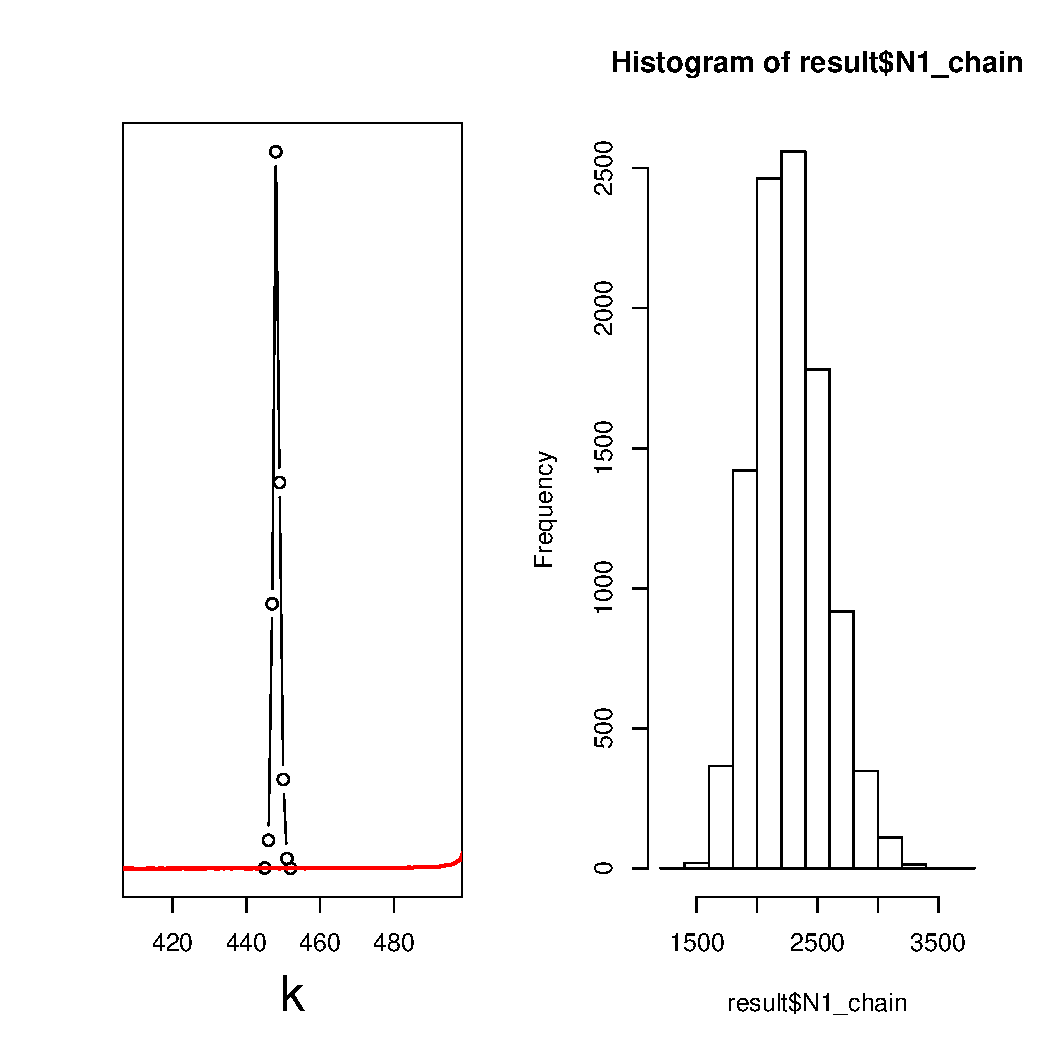
\includegraphics[width = \linewidth]{reFigure2.pdf}
    \caption{Posterior samples of cluster size and population size after running 10000 iterations of the coupled Gibbs sampler described in Section 2.}
    \label{fig:reproduce}
\end{figure}



\begin{comment}
\section{Some notes on label-switching papers}
The problem of label switching appears when both the likelihood function and the prior is symmetric with respect to all mixture components. This leads to a highly mutimodal symmetric posterior distribution that is difficult to summarize. For example, posterior mean does not have a natural interpretation. A common approach for tackling this problem is putting identifiability constraints on the prior that in turn imply constraints on the posterior.
As shown by \cite{stephens2000dealing} imposing identifiability constraints does not always solve the problem, the problem of multimodality stays. The approach of \cite{stephens2000dealing} addresses this problem from a decision-theoretic perespective. That is, it attempts to find the relabeling that minimizes a prespecified risk function.

\cite{jasra2005markov} gives a review of MCMC samplers and solutions to label-switching problems.

\end{comment}

\bibliographystyle{ba}
\bibliography{references_discussion}
\end{document}
